\documentclass[12pt]{article}

% for using MikTex latex and then creating a ps or pdf from the dvi file
% you might need to uncomment the following line
% \special{landscape} 

%%% load sslides.sty
\usepackage{sslides}

%%% to support German characters like ��� 
%\usepackage[]{fontenc}
%\usepackage[latin1]{inputenc} 
%\usepackage[austrian]{babel}

%%% graphics
\usepackage{graphicx}
\usepackage{mathtools}

%%%%%%%%%%%%%%%%%%%%%%%%%%%%%%%%%%%%%%%%%%%%%%%%%%%%%%%%%%%%%%%%%%%
%%% Change author info here
\def\nameTitle{Dan Kapner}
\def\emailTitle{danielk@alleninstitutue.org}

%%% Change presentation info
\def\presentationTitle{Simple 4 tile example for solver}

%%% used for footer in fancy headings
\def\nameFooter{\nameTitle}

%%%%%%%%%%%%%%%%%%%%%%%%%%%%%%%%%%%%%%%%%%%%%%%%%%%%%%%%%%%%%%%%%%%
% comment if fancyheadings.sty is not installed (e.g., for MikTex)
% you can change the logo in the file fancyheadings.tex
% %%% fancyheadings
\usepackage{fancyheadings}
\pagestyle{fancy}

% header
\lhead{} 
\chead{}

%%% logo
\rhead{\vspace{0.5cm}%
\includegraphics[height=1.2cm, width=1.2cm]{logos/wulogo}%
\includegraphics[height=1.2cm, width=1.7cm]{logos/ai-logo}}
%\rhead{}

%%% footer
\footrulewidth 0pt 
\headrulewidth 0pt
\rfoot{\footnotesize \placeAndDayFooter}
\lfoot{\footnotesize \nameFooter}
\cfoot{\footnotesize \thepage}


% \input{includes/fancyhdr}

%%% most beamers can't project decent colors so I set them to max!
% redefine emph color
%\definecolor{Emph}{rgb}{1,0,0}  %red
\definecolor{Emph}{rgb}{0.8,0.2,0.2}  %softer red for display
\renewcommand{\emph}[1]{\textcolor{Emph}{\bf\textit{#1}}}

% define color for slide titles
%\definecolor{Title}{rgb}{0,0,1}  %blue
\definecolor{Title}{rgb}{0.2,0.2,0.8}  %softer blue for display
%\definecolor{Title}{rgb}{1,0,0}  %red

%%%%%%%%%%%%%%%%%%%%%%%%%%%%%%%%%%%%%%%%%%%%%%%%%%%%%%%%%%%%%%%%%%%
\begin{document}
%%% Title slide: choose a title slide layout
%%% you can also adapt the title slide in includes/titlepage_...
%%% add entry for Titleslide
\addcontentsline{toc}{subsection}{\protect\numberline{\thesection}Title slide}%

%% Title slide

\phantom{.}\vspace{3cm}
{\LARGE \raggedright \textcolor{Title}{\bf \presentationTitle}} \\[3mm]
\textcolor{Title}{\presentationSubTitle}
\vspace{1cm}

\raggedright {\bf \nameTitle} \\[2mm]
{\small\affiliationTitle}
\vspace{1cm}

\raggedright {\small \eventTitle}
\raggedright {\small \placeAndDayTitle}

\thispagestyle{empty}



%%% add entry for Titleslide
\addcontentsline{toc}{subsection}{\protect\numberline{\thesection}Title slide}%

%% Title slide

\phantom{.}\vspace{3cm}
\begin{center}
{\LARGE \textcolor{Title}{\bf \presentationTitle}} \\[3mm]
\textcolor{Title}{\presentationSubTitle}
\vspace{1cm}

{\bf \name} \\[2mm]
{\small\affiliationTitle}
\vspace{1cm}

{\small \eventTitle}
{\small \placeAndDayTitle}

\end{center}
\thispagestyle{empty}



%% edit the logos in includes/titlepage_logo.tex
%%% add entry for Titleslide
\addcontentsline{toc}{subsection}{\protect\numberline{\thesection}Title slide}%

%% Title slide


\raggedleft 
\includegraphics[width=2.5cm]{logos/wulogo}
\includegraphics[width=3.2cm]{logos/ai-logo}
\vspace{2cm}

\raggedright \textcolor{Title}{\LARGE\bf \presentationTitle} \\[3mm]
\textcolor{Title}{\presentationSubTitle}

\vspace{1cm}

\raggedright {\bf \nameTitle} \\[2mm]
{\small\affiliationTitle}
\vspace{1cm}

\raggedright {\small \eventTitle}
\raggedright {\small \placeAndDayTitle}

\thispagestyle{empty}


 
	   
%%%%%%%%%%%%%%%%%%%%%%%%%%%%%%%%%%%%%%%%%%%%%%%%%%%%%%%%%%%%%%%%%%%%
%%% start with the slides here using sections and subsections as slides

\section{4tile example}
small example\\
\begin{itemize}
\item{understand matrix construction, code and linear algebra}
\end{itemize}
Dan Kapner\\
10/2/2017

\section{Source of Data}
%\begin{minipage}[m]{.9\textwidth}
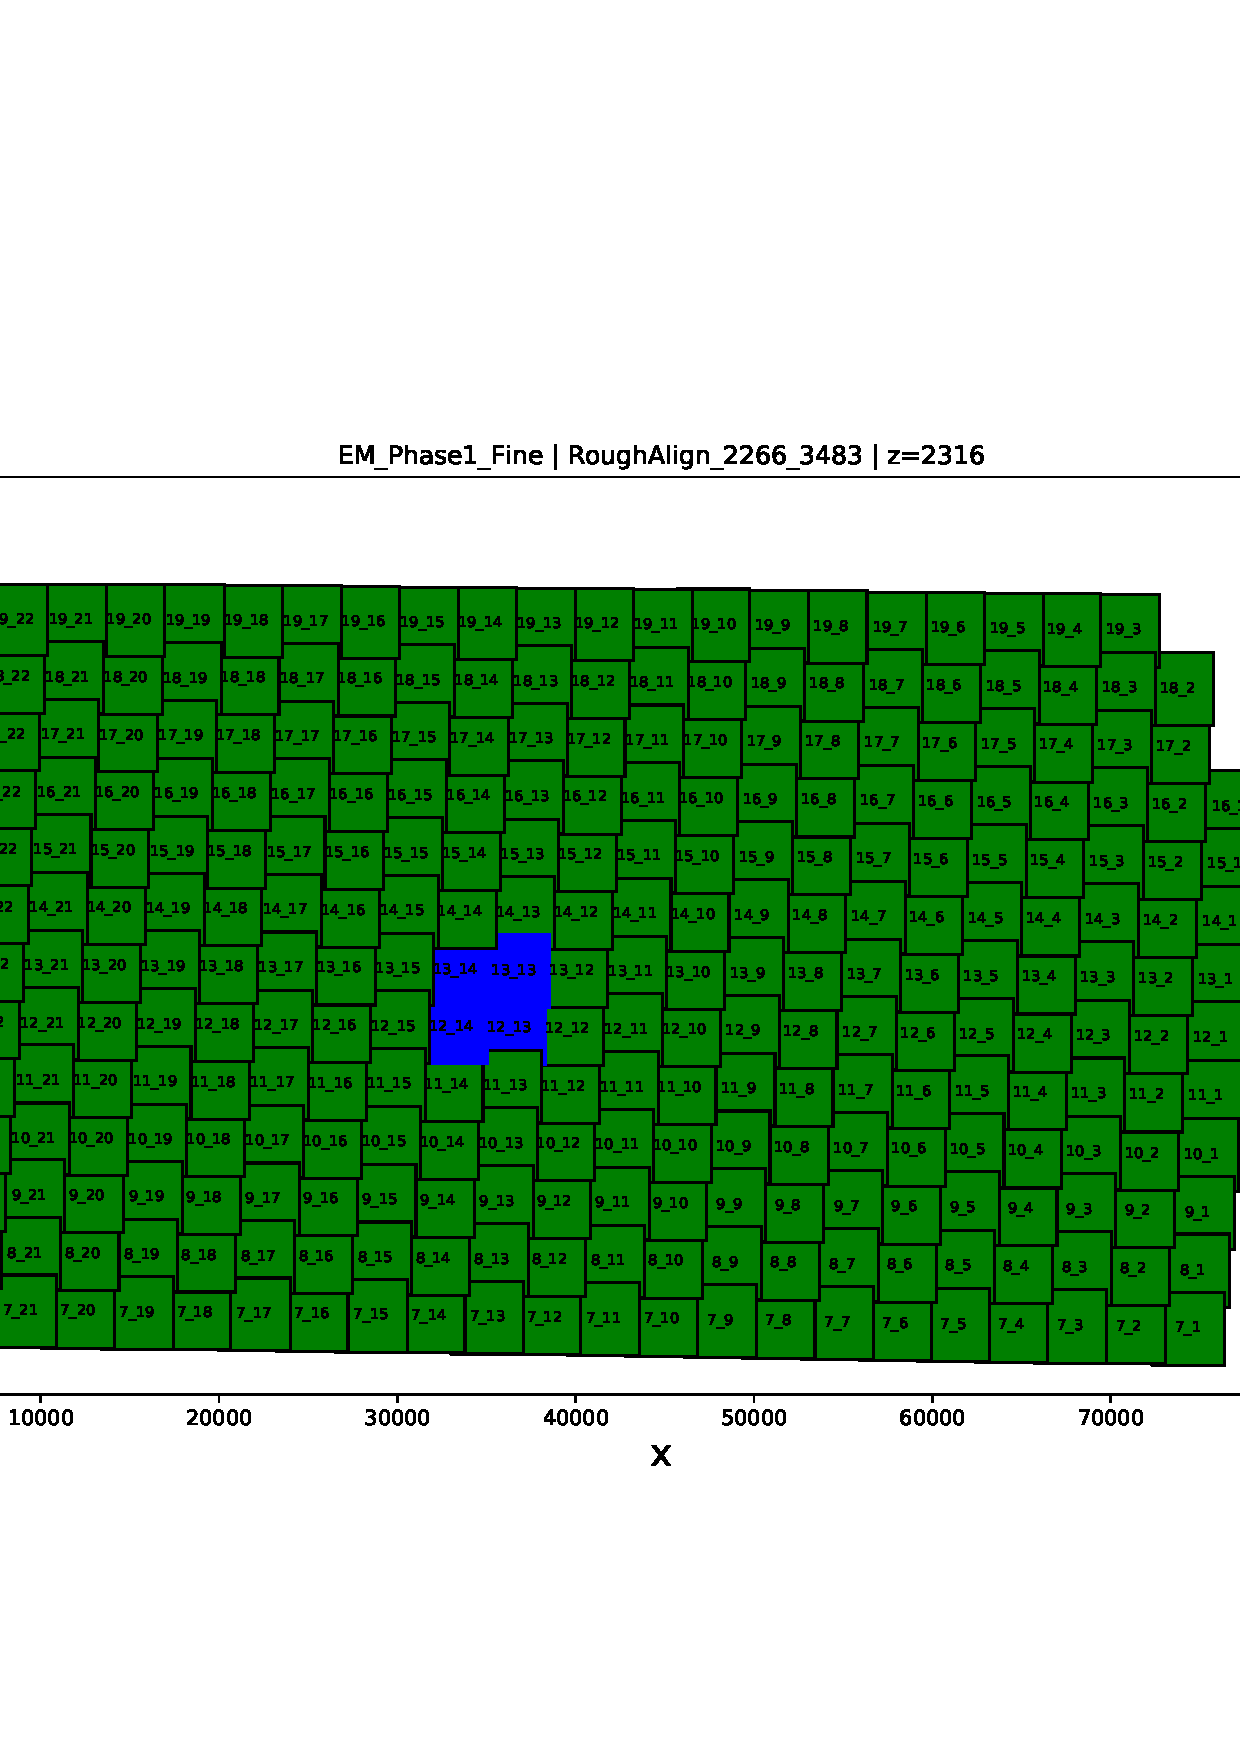
\includegraphics[width=7in]{figures/Section.pdf}
%\end{minipage}

\section{4 tiles and point matches}
\begin{minipage}[m]{.49\textwidth}
\includegraphics[width=7in]{figures/4tile_PM.pdf}
\end{minipage}

\section{Filtering}
%\begin{minipage}[m]{.49\textwidth}
\includegraphics[width=4in]{figures/matlab_filter.png}
%\end{minipage}
%\begin{minipage}[m]{.49\textwidth}
\includegraphics[width=4in]{figures/matlab_filter2.png}
%\end{minipage}
MATLAB filters down the pointmatch collection from 200 points per tile pair to around 50\\
There is some random aspect to the filtering.

\section{Naming and algebra}
%\begin{minipage}[m]{.49\textwidth}
%\includegraphics[width=4in]{figures/matlab_filter2.png}
%\end{minipage}

\begin{table}
\begin{tabular}{c|c}
tile 1 & tile 2\\
\hline
$(\prescript{1}{}{x}_1,\prescript{1}{}{y}_1)$ & $(\prescript{2}{}{x}_1,\prescript{2}{}{y}_1)$\\
$(\prescript{1}{}{x}_2,\prescript{1}{}{y}_2)$ & $(\prescript{2}{}{x}_2,\prescript{2}{}{y}_2)$\\
$(\prescript{1}{}{x}_3,\prescript{1}{}{y}_3)$ & $(\prescript{2}{}{x}_3,\prescript{2}{}{y}_3)$\\
$(\prescript{1}{}{x}_4,\prescript{1}{}{y}_4)$ & $(\prescript{2}{}{x}_4,\prescript{2}{}{y}_4)$\\
... & ...
\end{tabular}
\end{table}

affine transformation
\begin{equation}
\prescript{1}{}{u}_1=a_1\prescript{1}{}{x}_1+b_1\prescript{1}{}{y}_1+c_1
\end{equation}
\begin{equation}
\prescript{1}{}{v}_1=d_1\prescript{1}{}{x}_1+e_1\prescript{1}{}{y}_1+f_1
\end{equation}\\
requirement for alignment
\begin{equation}
\prescript{1}{}{u}_1=\prescript{2}{}{u}_1
\end{equation}
\begin{equation}
\prescript{1}{}{v}_1=\prescript{2}{}{v}_1
\end{equation}
explicitly
\begin{equation}
a_1\prescript{1}{}{x}_1+b_1\prescript{1}{}{y}_1+c_1=a_2\prescript{2}{}{x}_1+b_2\prescript{2}{}{y}_1+c_2
\end{equation}
\begin{equation}
d_1\prescript{1}{}{x}_1+e_1\prescript{1}{}{y}_1+f_1=d_2\prescript{2}{}{x}_1+e_2\prescript{2}{}{y}_1+f_2
\end{equation}
and in matrix form, this is:
\setcounter{MaxMatrixCols}{20}
\begin{tiny}
$$
\begin{bmatrix}
-\prescript{1}{}{x}_1 & -\prescript{1}{}{y}_1 & -1 & \prescript{2}{}{x}_1 & \prescript{2}{}{y}_1 & 1 & 0 & 0 & 0 & 0 & 0 & 0\\
0 & 0 & 0 & 0 & 0 & 0 & -\prescript{1}{}{x}_1 & -\prescript{1}{}{y}_1 & -1 & \prescript{2}{}{x}_1 & \prescript{2}{}{y}_1 & 1
\end{bmatrix}
\times
\begin{bmatrix}
a_1\\b_1\\c_1\\a_2\\b_2\\c_2\\
d_1\\e_1\\f_1\\d_2\\e_2\\f_2\\
\end{bmatrix}
=
\begin{bmatrix}
0\\
0\\
\end{bmatrix}
$$
\end{tiny}

and, now scaling to more than 1 point match pair:
\begin{tiny}
$$
\begin{bmatrix}
-\prescript{1}{}{x}_1 & -\prescript{1}{}{y}_1 & -1 & \prescript{2}{}{x}_1 & \prescript{2}{}{y}_1 & 1 & 0 & 0 & 0 & 0 & 0 & 0\\
-\prescript{1}{}{x}_2 & -\prescript{1}{}{y}_2 & -1 & \prescript{2}{}{x}_2 & \prescript{2}{}{y}_2 & 1 & 0 & 0 & 0 & 0 & 0 & 0\\
-\prescript{1}{}{x}_3 & -\prescript{1}{}{y}_3 & -1 & \prescript{2}{}{x}_3 & \prescript{2}{}{y}_3 & 1 & 0 & 0 & 0 & 0 & 0 & 0\\
-\prescript{1}{}{x}_4 & -\prescript{1}{}{y}_4 & -1 & \prescript{2}{}{x}_4 & \prescript{2}{}{y}_4 & 1 & 0 & 0 & 0 & 0 & 0 & 0\\
 &  & & ... \\
0 & 0 & 0 & 0 & 0 & 0 & -\prescript{1}{}{x}_1 & -\prescript{1}{}{y}_1 & -1 & \prescript{2}{}{x}_1 & \prescript{2}{}{y}_1 & 1\\
0 & 0 & 0 & 0 & 0 & 0 & -\prescript{1}{}{x}_2 & -\prescript{1}{}{y}_2 & -1 & \prescript{2}{}{x}_2 & \prescript{2}{}{y}_2 & 1\\
0 & 0 & 0 & 0 & 0 & 0 & -\prescript{1}{}{x}_3 & -\prescript{1}{}{y}_3 & -1 & \prescript{2}{}{x}_3 & \prescript{2}{}{y}_3 & 1\\
0 & 0 & 0 & 0 & 0 & 0 & -\prescript{1}{}{x}_4 & -\prescript{1}{}{y}_4 & -1 & \prescript{2}{}{x}_4 & \prescript{2}{}{y}_4 & 1\\
 &&&&&&&&...
\end{bmatrix}
\times
\begin{bmatrix}
a_1\\b_1\\c_1\\a_2\\b_2\\c_2\\
d_1\\e_1\\f_1\\d_2\\e_2\\f_2\\
\end{bmatrix}
=
\begin{bmatrix}
0\\0\\0\\0\\...\\0\\0\\0\\0\\...
\end{bmatrix}
$$
\end{tiny}

we can rearrange the columns to keep all the tile coordinates in one place:
\begin{tiny}
$$
\begin{bmatrix}
-\prescript{1}{}{x}_1 & -\prescript{1}{}{y}_1 & -1 & 0 & 0 & 0 & \prescript{2}{}{x}_1 & \prescript{2}{}{y}_1 & 1 & 0 & 0 & 0\\
-\prescript{1}{}{x}_2 & -\prescript{1}{}{y}_2 & -1 & 0 & 0 & 0 & \prescript{2}{}{x}_2 & \prescript{2}{}{y}_2 & 1 & 0 & 0 & 0\\
-\prescript{1}{}{x}_3 & -\prescript{1}{}{y}_3 & -1 & 0 & 0 & 0 & \prescript{2}{}{x}_3 & \prescript{2}{}{y}_3 & 1 & 0 & 0 & 0\\
-\prescript{1}{}{x}_4 & -\prescript{1}{}{y}_4 & -1 & 0 & 0 & 0 & \prescript{2}{}{x}_4 & \prescript{2}{}{y}_4 & 1 & 0 & 0 & 0\\
 &  & & ... \\
0 & 0 & 0 &  -\prescript{1}{}{x}_1 & -\prescript{1}{}{y}_1 & -1 &0 & 0 & 0 &  \prescript{2}{}{x}_1 & \prescript{2}{}{y}_1 & 1\\
0 & 0 & 0 &  -\prescript{1}{}{x}_2 & -\prescript{1}{}{y}_2 & -1 &0 & 0 & 0 &  \prescript{2}{}{x}_2 & \prescript{2}{}{y}_2 & 1\\
0 & 0 & 0 &  -\prescript{1}{}{x}_3 & -\prescript{1}{}{y}_3 & -1 &0 & 0 & 0 &  \prescript{2}{}{x}_3 & \prescript{2}{}{y}_3 & 1\\
0 & 0 & 0 &  -\prescript{1}{}{x}_4 & -\prescript{1}{}{y}_4 & -1 &0 & 0 & 0 &  \prescript{2}{}{x}_4 & \prescript{2}{}{y}_4 & 1\\
 &&&&&&&&...
\end{bmatrix}
\times
\begin{bmatrix}
a_1\\b_1\\c_1\\d_1\\e_1\\f_1\\
a_2\\b_2\\c_2\\d_2\\e_2\\f_2\\
\end{bmatrix}
=
\begin{bmatrix}
0\\0\\0\\0\\...\\0\\0\\0\\0\\...
\end{bmatrix}
$$
\end{tiny}

this is starting to look like Khaled's presentation.\\
change all the signs (absorb into the a,b,c,d parameters)\\
$$
\begin{bmatrix}
\prescript{1,2}{}{P} & -\prescript{1,2}{}{Q}\\
\end{bmatrix}
\times
\begin{bmatrix}
T_1\\T_2
\end{bmatrix}
=
\begin{bmatrix}
0\\0
\end{bmatrix}
$$

where, for example
$$
\begin{bmatrix}
\prescript{1,2}{}{P}
\end{bmatrix}
=
\begin{bmatrix}
-\prescript{1}{}{x}_1 & -\prescript{1}{}{y}_1 & -1 & 0 & 0 & 0 \\
-\prescript{1}{}{x}_2 & -\prescript{1}{}{y}_2 & -1 & 0 & 0 & 0 \\
-\prescript{1}{}{x}_3 & -\prescript{1}{}{y}_3 & -1 & 0 & 0 & 0 \\
-\prescript{1}{}{x}_4 & -\prescript{1}{}{y}_4 & -1 & 0 & 0 & 0 \\
... \\
0 & 0 & 0 &  -\prescript{1}{}{x}_1 & -\prescript{1}{}{y}_1 & -1 \\
0 & 0 & 0 &  -\prescript{1}{}{x}_2 & -\prescript{1}{}{y}_2 & -1 \\
0 & 0 & 0 &  -\prescript{1}{}{x}_3 & -\prescript{1}{}{y}_3 & -1 \\
0 & 0 & 0 &  -\prescript{1}{}{x}_4 & -\prescript{1}{}{y}_4 & -1 \\
 &&&...
\end{bmatrix}
$$

and 
$$
T_1=
\begin{bmatrix}
a_1\\b_1\\c_1\\d_1\\e_1\\f_1\\
\end{bmatrix}
$$

and where the following is a column-wise concatenation
$$
\begin{bmatrix}
\prescript{1,2}{}{P} & -\prescript{1,2}{}{Q}\\
\end{bmatrix}
$$
and where the following is a row-wise concatenation
$$
\begin{bmatrix}
T_1\\T_2
\end{bmatrix}
$$

this equation,again, is for 2 tiles:
$$
\begin{bmatrix}
\prescript{1,2}{}{P} & -\prescript{1,2}{}{Q}\\
\end{bmatrix}
\times
\begin{bmatrix}
T_1\\T_2
\end{bmatrix}
=
\begin{bmatrix}
0\\0
\end{bmatrix}
$$

when we expand it to 3 tiles\\
(with overlaps 1-2, 1-3, but not 2-3)
$$
\begin{bmatrix}
\prescript{1,2}{}{P} & -\prescript{1,2}{}{Q} & 0\\
\prescript{1,3}{}{P} & 0 & -\prescript{1,3}{}{Q}\\
\end{bmatrix}
\times
\begin{bmatrix}
T_1\\T_2\\T_3
\end{bmatrix}
=
\begin{bmatrix}
0\\0\\0
\end{bmatrix}
$$
and to 4 tiles\\
(with overlaps 1-2, 1-3, 2-4, 3-4, but not 1-4, 2-3)
$$
\begin{bmatrix}
\prescript{1,2}{}{P} & -\prescript{1,2}{}{Q} & 0 & 0\\
\prescript{1,3}{}{P} & 0 & -\prescript{1,3}{}{Q} & 0\\
 %0 & \prescript{2,3}{}{P} & -\prescript{2,3}{}{Q} & 0\\
 0 & \prescript{2,4}{}{P} & 0 &-\prescript{2,4}{}{Q} \\
 0 & 0 & \prescript{3,4}{}{P} & -\prescript{3,4}{}{Q} \\
\end{bmatrix}
\times
\begin{bmatrix}
T_1\\T_2\\T_3\\T_4
\end{bmatrix}
=
\begin{bmatrix}
0\\0\\0\\0
\end{bmatrix}
$$

Let's cut the point-matches per tile pair down to 10, so it is easier to see this same structure in the example. Below is structure plot and value-coded, to see the repeating structure.

\includegraphics[width=7in]{figures/10pm_structure.png}

based on the looks of this, the row ordering is a little different than the example above.\\
It's fine, because we're just re-ordering zeros on the right-hand side.\\
 Instead, we are seeing:

$$
\begin{bmatrix}
\prescript{1,3}{}{P} & 0 & -\prescript{1,3}{}{Q} & 0\\
0 & 0 & \prescript{3,4}{}{P} & -\prescript{3,4}{}{Q}\\
\prescript{1,2}{}{P} & -\prescript{1,2}{}{Q} & 0 & 0\\
 0 & \prescript{2,4}{}{P} & 0 &-\prescript{2,4}{}{Q} \\
\end{bmatrix}
\times
\begin{bmatrix}
T_1\\T_2\\T_3\\T_4
\end{bmatrix}
=
\begin{bmatrix}
0\\0\\0\\0
\end{bmatrix}
$$
\begin{equation}
\left(Ax=b\right)
\end{equation}

The transforms we are solving for:
$$
\begin{bmatrix}
T_1\\T_2\\T_3\\T_4
\end{bmatrix}
$$
represent 24 unknowns.\\
The matrix has 80 rows.\\
The system is overdetermined.\\
We want a solution for $x$ which minimizes the norm of the residuals:\\
\begin{equation}
S(x) = ||b-Ax||^2
\end{equation}
There are a few forms of this (see wikipedia: normal equations), but, I think this one makes it clear.\\
A is $m$x$n$
\begin{equation}
r_i = b_i-\sum_{j=1}^{n}A_{ij}x_j
\end{equation}
\begin{equation}
S=\sum_{i=1}^{m}r_i^2
\end{equation}
minimize with respect to x to find the best fit:
\begin{equation}
\frac{\partial{S}}{\partial{x_j}}=2\sum_{i}^{m}r_i\frac{\partial{r_i}}{x_j}
\end{equation}
\begin{equation}
\frac{\partial{r_i}}{x_j}=-A_{ij}
\end{equation}
\begin{equation}
\frac{\partial{S}}{\partial{x_j}}=2\sum_{i}^{m}\left(b_i-\sum_{k=1}^{n}A_{ik}x_k\right)\left(-A_{ij}\right)=0
\end{equation}
rearranging:
\begin{equation}
\sum_{i=1}^{m}\sum_{k=1}^{n}A_{ij}A_{ik}x_k = \sum_{i=1}^{m}A_{ij}b_i
\end{equation}
which is:
\begin{equation}
A^TAx=A^Tb
\end{equation}
$A^TA$ is $n$x$n$, so, now we have n equations and n unknowns.
The solver includes a way to weight points differently. In this example, this means including an 80x80 diagonal matrix, $W$:
\begin{equation}
A^TWAx=A^TWb
\end{equation}
For equal weighting, $W=I$.\\
The solver also includes regularization:
\begin{equation}
A^TWAx+\lambda=A^TWb+\lambda  d
\end{equation}
or
\begin{equation}
Kx=L_m
\end{equation}
where $K$ is square, and $L_m$ has non-zero entries:
\includegraphics[width=7in]{figures/10pm_Kstructure.png}
Looking at the graph of K, it shows two disconnected graphs. 
\includegraphics[width=7in]{figures/Kgraph.png}
We can use this to permute the rows and columns, to get:
\includegraphics[width=7in]{figures/reorder.png}\\
This permuted structure plot implies an obvious way to partition the matrix for distributed solving.
\\Let's go bigger. A whole section (282 tiles):\\
\includegraphics[width=8in]{figures/wholesection.png}
now, let's add a second section:\\
\includegraphics[width=8in]{figures/2sections.png}
now, 10 sections:\\
\includegraphics[width=8in]{figures/10sections.png}
22 sections from EM\_Phase1\_Fine is the most I can run through right now (unknown code crash):\\
\includegraphics[width=8in]{figures/22sections.png}



\end{document}

